\documentclass{article}
\usepackage{german}

\setlength{\emergencystretch}{15pt}

\usepackage{graphicx}

\usepackage{amsmath}

\begin{document}

\section{Herleitung}

\subsection{Methode}
\paragraph{Start}
$z_k^{(i)} = x;z_k^{(i+1)} = y$ in die Weierstraß-Iteration einsetzen 
\begin{equation}
    g(x) = y = x - \frac{p(x)}{\prod_{j=1;j\neq k}^{n} (x-z_j^{(i)})}
\end{equation}
Graph angucken (Beispiel)
\begin{figure}[h]
    \centering
    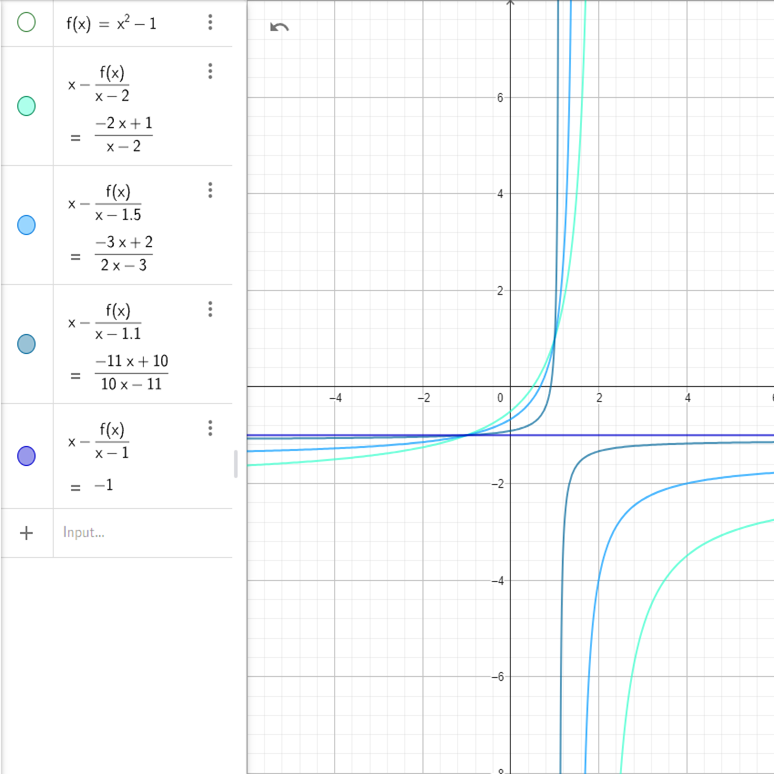
\includegraphics[scale=.6]{BeispielHerleitung.png}
    \caption{Beispiel: $x^2-1$ für die Nullstelle $-1$}
\end{figure}
%-------------------------------------------------------------------------------------------------------------------
\paragraph{Wenn alle Nullstellen gefunden konstant} Irrelevant
Falls die restlichen Nullstellen gefunden wurden waagrechte Gerade -> Für jeden Wert $z_k^(i)$ kommt die Nullstelle $z_k$ raus
Nicht zu beachten, da die exakte Nullstelle erst im unendlichen gefundne wird
\begin{align*}
    y &= x - \frac{p(x)}{\prod_{j=1;j\neq k}^{n} (x-z_j)} \\
    &= x - (x-z_k) \\
    &= z_k
\end{align*}
%-------------------------------------------------------------------------------------------------------------------
\paragraph{Nicht der Fall}
Sonst gebrochen rationale Funktion
%-------------------------------------------------------------------------------------------------------------------
\subparagraph{Vergleich mit waagrechten}
Diese verläuft ähnlich die die waagrechte, allerdings hat Definitionslücken und ist um diese \glqq verfälscht\grqq. Diese \glqq Verfälschung\grqq\space nimmt mit steigendem Abstand zu der Definitionslücke ab, da der gebrochene Term der Funktion immer kleiner wird. 
$g(z_k) = z_k$
%-------------------------------------------------------------------------------------------------------------------
\subparagraph{Verhalten im unendlichen}
Gleichung (1) hat, wenn die Nullstellen nicht stimmen, eine waagrechte Asymptote. Das kann daran gesehen werden, dass der Grad des Nenners gleich des Grades des Zählers ist. Das sieht man, durch ein wenig umstellen:
\begin{align*}
    ?
\end{align*}
Daran sieht man dass im negativen unendlichen $y < x$ ist
In richtung minus Unendlich fällt Von $z_k$ aus
Bedeutet, dass $z_k^{(i+1)}$ näher an der Nullstelle ist als $z_k^{(i)}$
%-------------------------------------------------------------------------------------------------------------------
\subparagraph{verhalten vor der nullstelle}
betrag immer größer als nullstelle -> geht nicht über die nullstelle hinaus
%-------------------------------------------------------------------------------------------------------------------
\subparagraph{verhalten nach der nullstelle}
betrag immer größer als nullstelle -> geht nicht über die nullstelle hinaus
%-------------------------------------------------------------------------------------------------------------------
\subparagraph{verhalten auf der Nullstelle}
$g(z_k) = z_k$
%-------------------------------------------------------------------------------------------------------------------
\paragraph{Außnahmen und Probleme}
Definitionslücken


\end{document}